\documentclass{report}

\usepackage{amsmath, amsthm, amssymb, amsfonts}
\usepackage{thmtools}
\usepackage{graphicx}
\usepackage{subcaption}
\usepackage{setspace}
\usepackage{geometry}
\usepackage{float}
\usepackage{hyperref}
\usepackage[utf8]{inputenc}
\usepackage[english]{babel}
\usepackage{framed}
\usepackage[dvipsnames]{xcolor}
\usepackage{tcolorbox}
\usepackage{multicol}
\usepackage{wrapfig}
\usepackage{minted}

\colorlet{LightGray}{White!90!Periwinkle}
\colorlet{LightOrange}{Orange!15}
\colorlet{LightGreen}{Green!15}

\newcommand{\HRule}[1]{\rule{\linewidth}{#1}}

\declaretheoremstyle[name=Theorem,]{thmsty}
\declaretheorem[style=thmsty,numberwithin=section]{theorem}
\tcolorboxenvironment{theorem}{colback=LightGray}

\declaretheoremstyle[name=Proposition,]{prosty}
\declaretheorem[style=prosty,numberlike=theorem]{proposition}
\tcolorboxenvironment{proposition}{colback=LightOrange}

\declaretheoremstyle[name=Principle,]{prcpsty}
\declaretheorem[style=prcpsty,numberlike=theorem]{principle}
\tcolorboxenvironment{principle}{colback=LightGreen}

\setstretch{1.2}
\geometry{
    textheight=9in,
    textwidth=5.5in,
    top=1in,
    headheight=12pt,
    headsep=25pt,
    footskip=30pt
}

% ------------------------------------------------------------------------------
\tcbset{
    sharp corners,
    colback = white,
    before skip = 0.2cm,    % add extra space before the box
    after skip = 0.5cm      % add extra space after the box
}                           % setting global options for tcolorbox

\definecolor{main}{HTML}{5989cf}    % setting main color to be used
\definecolor{sub}{HTML}{cde4ff}     % setting sub color to be used

\newtcolorbox{boxH}{
    colback = sub, 
    colframe = main, 
    boxrule = 0pt, 
    leftrule = 6pt % left rule weight
}

\newcommand{\SubItem}[1]{
    {\setlength\itemindent{15pt} \item[-] #1}
}

% ------------------------------------------------------------------------------

\begin{document}

% ------------------------------------------------------------------------------
% Cover Page and ToC
% ------------------------------------------------------------------------------

\title{ \normalsize \textsc{}
		\\ [2.0cm]
		\HRule{1.5pt} \\
    \LARGE \textbf{\uppercase{Advanced Information System Security}}
		\HRule{2.0pt} \\ [0.6cm] \LARGE{Hoping to get a better grade this time around.} \vspace*{10\baselineskip}}
\author{\textbf{Fabio Lorenzato}} 
		

\maketitle
\newpage

\tableofcontents
\newpage
\chapter{Transport Layer Security}
TLS, or Transport Layer Security, was originally proposed by Netscape
in 1995 as a way to secure communications between a web browser and a
web server. It is the successor to SSL, or Secure Sockets Layer, which
was first introduced by Netscape in 1995. The two terms are often used
interchangeably, but TLS is the more modern and secure protocol.\\ 
The main goal of SSL was to create secure transport channel, almost at
session level(4.5), between two parties, to provide some security
services:
\begin{itemize}
  \item \textbf{peer authentication} based on asymmetric
    challenge-response authentication(the challenge for the service is
    implicit, while for the client is explicit)
  \item \textbf{message confidentiality} base on symmetric encryption
  \item message integrity and authentication based on MAC
  \item replay, filtering and reordering attack protection using
    implicit record numbers( the correct order of transmission is
    provided by TCP, for this reason the number is implicit). This
    number is used also in the MAC computation.

\end{itemize}

You can see the TLS packet structure in figure
\ref{fig:tls-packet-structure}.
The TLS record protocol contains the generic protocols informations
and its content depend of the state of the connection and the protocol
it is tunneling.
\begin{figure}[H]
    \centering
    \includegraphics[width=.6\textwidth]{img/TLS packet
    structure.png}
    \caption{TLS packet structure.}
    \label{fig:tls-packet-structure}
\end{figure}

\section{TLS session and connection}
It is important to make a clear distinction between TLS session and
connections.

TLS sessions a logical association between client and server, created
via an handshake protocol and its shared between different TLS
connections(1:N).

TLS connections are a transient TLS channel between client and server,
which means that each connection is associated with only one specific
TLS session(1:1).
% Add image later
\section{TLS handshake protocol}
The TLS handshake protocol is used to establish a new session or
reestablish an existing session. During this phase the two parts agree
agree on a set of algorithms for confidentiality and integrity,
exchange random numbers between the client and the server to be used
for the subsequent generation of the keys, establish a symmetric key
by means of public key operations (RSA, DH, ...), negotiate the
session-id and exchange the necessary certificates.

\section{Achieving Data protection}
Data protection is achieved by using symmetric encryption algorithms
to encrypt the data and Message Authentication Codes(MAC) to ensure
the integrity of the data and the authentication of the sender.

\begin{figure}[H]
  \centering
  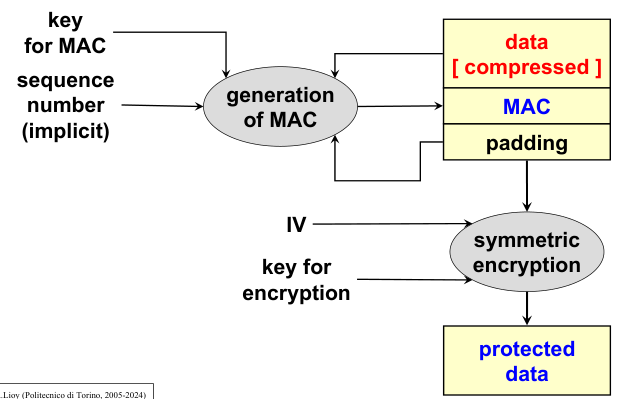
\includegraphics[width=.5\textwidth]{img/TLS data protection.png}
  \caption{TLS data protection.}
  \label{fig:tls-data-protection}
\end{figure}

The keys are direction, so there are two keys( one for client to
server and one for server to client) to protect against reuse of the
sequence number in the opposite direction.

\section{Perfect Forward Secrecy}
Since the keys are generated from asymmetric crypto, if the private
key is compromised, all the previous communication can be decrypted.
In this context, perfect forward secracy is desirable.
\begin{boxH}
  \textbf{Perfect Forward Secrecy} is a property of key-agreement
  protocols ensuring that the compromise of the secret key used for 
  will compromise only current (and eventually future) traffic but not
  the past one
\end{boxH}
The most common way to achieve this is to use ephiemeral keys, which
are one-time asymmetric keys( used for key exchange) 

\section{The protocol}
The TLS handshake is always initiated by the client. 

\subsection{Client Hello and Server Hello}
In version 1.2 the client sends a Client Hello, which contains:
\begin{itemize}
  \item the SSL version preferred by the client, and the highest
    supported(2=SSL-2, 3.0=SSL-3, 3.1=TLS-1.0, \dots)
  \item a 28 bytes pseudo-random number, which is the client random
  \item a session-id, which is empty if the client is starting a new
    session, and not empty if the client is trying to resume a 
    previous session
  \item a list of cipher suites supported by the client, in order to 
    let the server choose the most secure one.
  \item a list of compression methods supported by the client
\end{itemize}

And then a server hello is sent back, which contains:
\begin{itemize}
  \item the SSL version chosen by the server
  \item a 28 bytes pseudo-random number, which is the server random
  \item a session identifier(session-id), which is a new one if the
    server is starting a new session, and the same as the client's if
    the server is resuming a previous session
  \item the cipher suite chosen by the server, the strongest one
    common between the client and the server
  \item the compression method chosen by the server
\end{itemize}


\begin{figure}[H]
  \centering
  \begin{subfigure}{.5\textwidth}
    \centering
    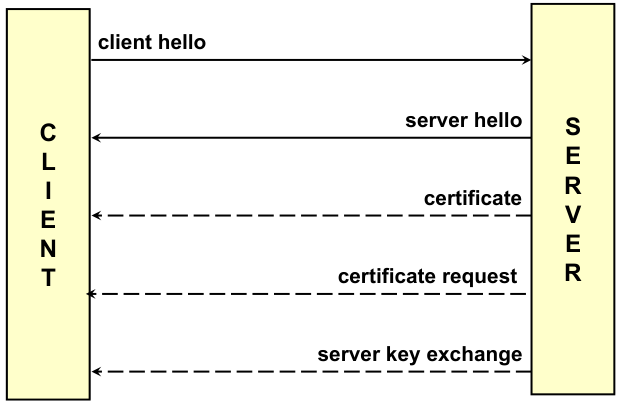
\includegraphics[width=.9\linewidth]{img/TLS key echange.png}
    \caption{The TLS handshake protocol(TLS 1.2).}
    \label{fig:tls-handshake-protocol-1.2}
  \end{subfigure}%
  \begin{subfigure}{.5\textwidth}
    \centering
    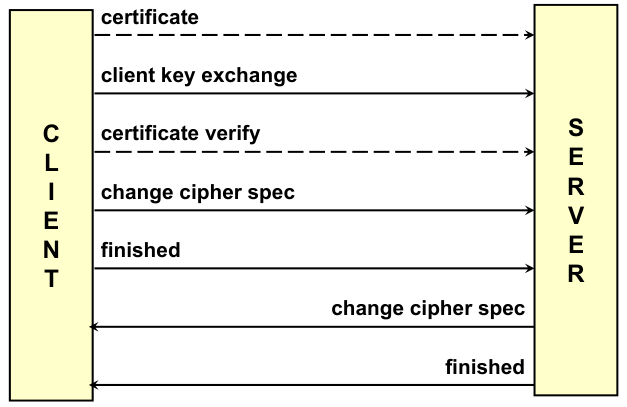
\includegraphics[width=.9\linewidth]{img/TLS key exchange 1-3.png}
    \caption{The TLS handshake protocol(TLS 1.3).}
    \label{fig:tls-handshake-protocol-1.3}
  \end{subfigure}
\end{figure}

\subsection{Cipher suite}
A cipher suite is a set of cryptographic algorithms used in the TLS
protocol. A typical cipher suite consists of a key exchange algorithm,
the symmetric encryption algorithm, and the hash function used for 
generating MACs.
Some example of those are:
\begin{itemize}
  \item SSL\_NULL\_WITH\_NULL\_NULL
  \item SSL\_RSA\_WITH\_NULL\_SHA
  \item SSL\_RSA\_EXPORT\_WITH\_RC2\_CBC\_40\_MD5
  \item SSL\_RSA\_WITH\_3DES\_EDE\_CBC\_SHA
\end{itemize}


\subsection{Certificates}
The server sends its certificate to the client for server
authentication.
% there should lie the server authentication even if ephimeral keys
% are not used

Optionally, the server can request a certificate from the client for
client authentication. In this case the server specifies the list of
trusted CA's, and the client sends its certificate chain. The browsers
show to the users (for a connection) only the certificates issued by
trusted CAs.
If client certificate verification is required, an explicit request to
send the hash computed over all the handshake messages before this 
one and encrypted with the client private key is sent to the client.

\subsection{Key exchange}
The key exchange is the most important part of the handshake protocol.
The server key exchange message is sent only if the

\subsection{Change cipher spec}
The change cipher spec message used to trigger the change of the
algorithms to be used for message protection. It allows to pass from
the previous unprotected messages to the protection of the next
messages with algorithms and keys just negotiated, thus is technically
a protocol on its own and not part of the handshake. Some analysis
even say that it could be removed from it.


\subsection{Finished message}
The finished message is the last message of the handshake protocol,
and the first message protected by the negotiated keys and algorithms.
It is necessary to ensure that the handshake has not been tampered
with, and it contains contains a MAC computed over all the previous
handshake messages (but change cipher spec) using as a key the master
secret. Notice that the finished message is different for the client 
and the server, because the MAC is computed over different messages.

This allows to prevent rollback man-in-the-middle attacks (version
downgrade or ciphersuite downgrade)

\section{Setup Time}
The setup time is the time required to establish a secure connection 
between the client and the server. TLS depends on TCP, so the TCP
handshake must be taken into account. Then the TLS handshake is
performed, meaning that typically 3 RTTs (1 for TCP and 2 for TLS) are
required to establish a secure connection. Usually after 180ms the two
parties are ready to send protected data( assuming 30ms delay
one-way).

\section{TLS versions}
\subsection{TLS 1.0}
TLS 1.0, or SSL 3.1, was released in 1999. It is the first version of
the protocol, and it is based on SSL 3.0. Previous version were using
proprietary solutions, so the adoption of open standards was strongly
encouraged.

\subsection{TLS 1.1}
TLS 1.1 was released in 2006, and it introduced some security fixes
especially to protect against CBC attacks. In fact, the implicit
IV is replaced with an explicit IV to protect against CBC attacks.
Also protection against padding oracle attacks were instroduces to
reduce the information leaks. For this reason Passing errors now use
the bad\_record\_mac alert message (rather than the decryption\_failed
one). Furthermore, premature closes no longer cause a session to be non-
resumable.

\subsection{TLS 1.2}
TLS 1.2 was released in 2008, and it introduced some new features and 
improvements. The chipersuite also specifies the pseudo random
function instead of leaving the choice to the implementation. The
sha-1 algorithm was replaced with SHA-256, and its also added support
for authenticated encryption, such as AES in GCN or CCM mode.

All the chipersuites tat use IDEA and DES are deprecated.

\section{TLS attacks}
\subsection{Heartbleed}
Heartbleed is a security bug in the OpenSSL cryptography library,
which is a widely used implementation of the TLS protocol. It was able
to exploit the fact that the heartbeat extension keeps the connection
alive without the need to negituate the SSL session again. The
attacker could send a heartbeat request, but the length of the 
response is much longer( up to 64KB) than the actual data sent by the
client. This attack could then allow to leak memory contents.

\subsection{Bleichenbacher attack}

\subsection{Other attacks against SSL/TLS}
Some other attacks against SSL/TLS are CRIME, BREACH, BEAST and
POODLE.\\
Crimes is an attack against the compression algorithm used in SSL/TLS,
which by injection chosen plaintext in the user requests and then
measure the size of the encrypted traffic, an attacker could recover
specific plaintext parts exploiting information leaked from the
compression, and this is part of the reason why the compression is
deprecated in TLS 1.3.\\
BREACH is an attack against the HTTP compression to deduce a secret
within the HTTP response provided by the server.\\
POODLE, or Padding Oracle On Downgraded Legacy Encryption, is an 
attack that exploits the fact that SSL 3.0 uses a padding scheme that
is vulnerable to a padding oracle attack, by acting as a MITM. This is
done by exploiting SSL-3 fallbacks to decrypt data.\\
For all those reasons SSL-3 has been disabled on most browsers, but
its still needed for some browsers, for example IE6 by Microsoft,
which is outlasting its expected life.

\subsection{FREAK attack}
FREAK, or Factoring RSA Export Keys, is an attack that exploits the
downgrades on TLS to explort-level RSA keys to a factorizable bit
length(512 bits). It is also possible to carry this out by downgrading
the symmetric key too and then perform a brute force attack( 40-bit).

\begin{figure}[H]
  \centering
  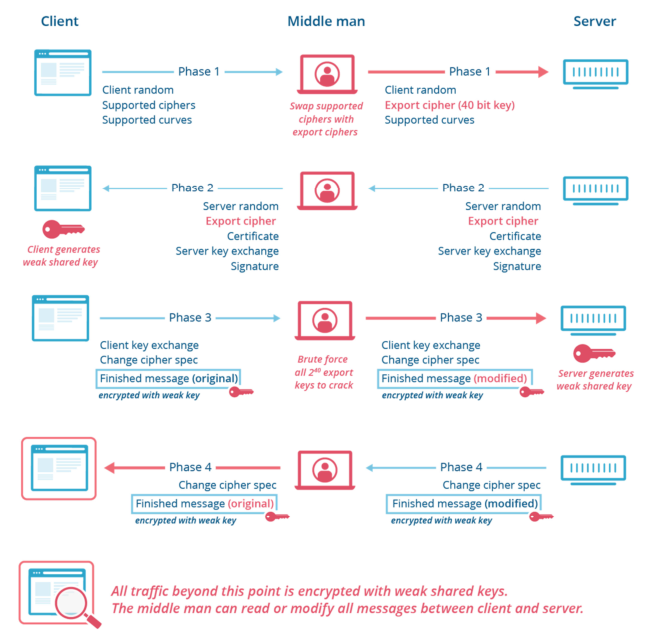
\includegraphics[width=.6\textwidth]{img/FREAK attack.png}
  \caption{FREAK attack.}
  \label{fig:freak-attack}
\end{figure}

\section{ALPN extension}
The ALPN extension, or Application-Layer Protocol Negotiation, is an
extension that allow to negotiate the application protocol to speed up
the connection creation, avoiding additional round- trips for
application negotiation. It is used to negotiate the protocol to be 
used on top of the TLS connection, such as HTTP/2, SPDY, or QUIC.
The extension is inserted in the client hello message, by setting the
ALPN flag to true and providing a list of supported protocols.
This is also useful for those servers that use different certificates
for the different application protocols.

\section{TLS False Start}
TLS False Start is another extension that allows the client can send
application data together with the ChangeCipherSpec and Finished
messages, in a single segment, without waiting for the corresponding
server messages. The biggest advantage of using this is the reduction
of the latency to 1 RTT. In theory this should work without changes,
but to use this in Chrome and Firefox they require the ALPN and the 
Forward Secrecy enabled, while Safari requires forward secrecy.

\section{The TLS downgrade problem}
In theory, when negotiating the TLS version to be used, the client
sends (in ClientHello) the highest supported version, while the server
notifies (in ServerHello) the version to be used (highest in common
with client)

\subsection{TLS Fallback Signalling Cipher Suite Value (SCSV)}
The TLS Fallback SCSV is a special value that is used to prevent 
the protocol downgrade attacks. It do so by sending a new (dummy)
ciphersuite value(TLS\_FALLBACK\_SCSV) which is sent by the client when
opening a downgraded connection )as last in the chipersuite list.

\section{TLS session tickets}
We know that session resumption is possible with TLS, but the server
needs to keep a cache of session IDs, which may become very large for
high traffic servers. For this reason, the TLS session tickets were
introduced, which are an extension allowing the server to send the
session data to the client encrypted with a server secret key. This
data is stored by the client, which will send it again when it wants
to resume a session. This allows to move the cache to the client side.

\section{The Virtual Server Problem}
Nowadays, virtual servers are very common in web hosting, because they
allows to have different logical names associated with the same IP
address( ie: home.myweb.it=10.1.2.3, food.myweb.it=10.1.2.3).
This is easy to manage in HTTP/1.1 but quite troublesome with HTTPS,
because TLS is activated before the HTTP request is sent, which makes
it difficult to know which certificate should be provided in advance.
The solutions are quire simple:
\begin{itemize}
  \item use a wildcard certificate, which is a certificate that is
    valid for all the subdomains of a domain (ie: *.myweb.it)
  \item use the SNI (Server Name Indication) extension, which is an
    extension that allows the client to specify the hostname of the
    server it is trying to connect to, allowing the server to provide
    the correct certificate. This is sent in the ClientHello message.
  \item provide a certificate with a list of servers in subjectAltName
\end{itemize}

\section{TLS 1.3}
TLS 1.3 was released in 2018, and it introduced some new features
while solving some of the most common problems of the previous 
versions:
\begin{itemize}
  \item reduce the handshake latency in general 
  \item encrypting more of the handshake (for security and privacy)
  \item improving resiliency to cross-protocol attacks
  \item removing legacy features
\end{itemize}
We will now go over the main changes in TLS 1.3.

\subsection{Key exchange}
In this version, the support for static RSA and DH key exchange was
removed for many reasons:
\begin{itemize}
  \item it does not implement forward secrecy 
  \item its difficult to implement correctly
\end{itemize}
Now Diffie-Hellman ephemeral (DHE) and Elliptic Curve Diffie-Hellman
Ephemeral (ECDHE) are the only key exchange methods supported, with
some required parameters.

\subsection{Message protection}

\subsection{Digital signature}

\subsection{Ciphersuites}
\begin{itemize}
  \item TLS\_AES\_128\_GCM\_SHA256
  \item TLS\_AES\_256\_GCM\_SHA384
  \item TLS\_CHACHA20\_POLY1305\_SHA256
  \item TLS\_AES\_128\_CCM\_SHA256
  \item TLS\_AES\_128\_CCM\_8\_SHA256 (deprecated)

\end{itemize}

\subsection{EdDSA}
EdDSA, or Edwards-curve Digital Signature Algorithm, is a digital 
signature scheme using the EdDSA signature scheme. The EdDSA scheme,
unlike standard DSA doesnt require a PRNG, which could in some cases
leak the private key if the underlying generation algorithm is broken
or predictable.\\
EdDSA picks a nonce based on a hash of the private key and the
message, which means after the private key is generated there’s no
more need for random number generators. Another advantage is that the
EdDSA is faster in signature generation and verification than the
standard DSA.


\subsection{Other improvements}

\subsection{HKDF in TLS 1.3}

\subsection{TLS-1.3 handshake}

\begin{figure}[H]
  \centering
  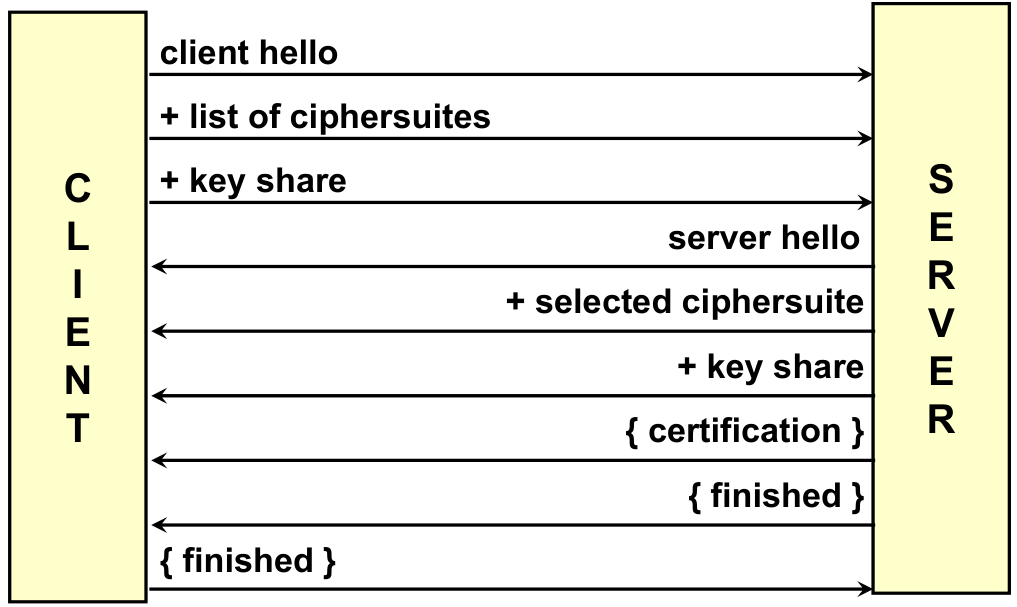
\includegraphics[width=.6\textwidth]{img/TLS 1-3 handshake.png}
  \caption{TLS 1.3 handshake.}
  \label{fig:tls-1.3-handshake}
\end{figure}

\subsection{Pre-shared keys}
In TLS, the pre-shared key (PSK) replaces the session ID and session
ticket. PSKs are agreed upon during a full handshake and can be reused
for multiple connections. They can be combined with (EC)DHE to achieve
forward secrecy, where the PSK is used for authentication and (EC)DHE
for key agreement. While PSKs can be generated out-of-band (OOB) from
a passphrase, this is risky due to the potential lack of randomness,
making brute-force attacks feasible. Therefore, using OOB PSKs is
generally discouraged.

\subsection{0-RTT connections}
In TLS 1.3, when using a pre-shared key (PSK), a client can send
"early data" with its initial message, which is protected by a
specific key. However, this approach lacks forward secrecy because it
relies solely on the PSK and could be vulnerable to replay attacks.
While some complex mitigations exist, they are particularly
challenging for multi-instance servers.

\subsection{Incorrect share}
In TLS 1.3, if a client sends a list of (EC)DHE groups that the server
does not support, the server responds with a HelloRetryRequest,
prompting the client to restart the handshake with different groups.
If the new groups are also unacceptable, the handshake will be
aborted, and the server will send an appropriate alert.

\end{document}
